\documentclass[12pt,letterpaper]{article}
\usepackage[utf8]{inputenc}
\usepackage[spanish]{babel}
\usepackage{graphicx}
\usepackage[left=2cm,right=2cm,top=2cm,bottom=2cm]{geometry}
\usepackage{graphicx} % figuras
% \usepackage{subfigure} % subfiguras
\usepackage{float} % para usar [H]
\usepackage{amsmath}
%\usepackage{txfonts}
\usepackage{stackrel} 
\usepackage{graphicx}
\usepackage{subfig}
\usepackage{hyperref}
\usepackage{multirow}
\usepackage{enumerate} % enumerados
\renewcommand{\labelitemi}{$-$}
\renewcommand{\labelitemii}{$\cdot$}
% \author{}
% \title{Caratula}
\begin{document}

% Fancy Header and Footer
% \usepackage{fancyhdr}
% \pagestyle{fancy}
% \cfoot{}
% \rfoot{\thepage}
%

% \usepackage[hidelinks]{hyperref} % CREA HYPERVINCULOS EN INDICE
  
% \author{}
\title{Caratula}

\begin{titlepage}
    \begin{center}
    \begin{figure}[htb]
    \begin{center}
    
\includegraphics[width=3.5cm]{./img/upt.jpg}
    \end{center}
    \end{figure}
    
    \vspace*{0.15in}
    \begin{Large}
    \textbf{UNIVERSIDAD PRIVADA DE TACNA}\\
    \end{Large}
    
    \vspace*{0.1in}
    \begin{Large}
    \textbf{FACULTAD DE INGENIERIA} \\
    \end{Large}
    
    \vspace*{0.1in}
    \begin{Large}
    \textbf{ESCUELA PROFESIONAL DE INGENIERIA DE SISTEMAS} \\
    \end{Large}
    
    \vspace*{0.5in}
    \begin{Large}
    \textbf{TITULO:}\\
    \end{Large}
    

\vspace*{0.1in}
\begin{Large}
    PRACTICA DE LABORATORIO 01: MODELAMIENTO DIMENSIONAL \\
\end{Large}

\vspace*{0.3in}
\begin{Large}
\textbf{Curso:} \\
\end{Large}

\vspace*{0.1in}
\begin{large}
    Inteligencia De Negocios\\
\end{large}

\vspace*{0.3in}
\begin{Large}
\textbf{Docente:} \\
\end{Large}

\vspace*{0.1in}
\begin{large}
Ing. Patrick Cuadros Quiroga\\
\end{large}

\vspace*{0.2in}
\vspace*{0.1in}
\begin{large}
\textbf{Alumno:} \\
\begin{flushleft}
 Herrera Amezquita, Derian Francisco		\hfill	(2017059489) \\


\end{flushleft}
\end{large}
\vspace*{0.1in}
\begin{large}
Tacna - Perú\\
\end{large}
\vspace*{0.1in}
\begin{large}
2021\\
\end{large}

\end{center}

\end{titlepage}



\tableofcontents % INDICE
\thispagestyle{empty} % INDICE SIN NUMERO
\newpage
\setcounter{page}{1} % REINICIAR CONTADOR DE PAGINAS DESPUES DEL INDICE


\section{Objetivos}
A.
\section{Requerimientos}
Conocimientos:
\\Para el desarrollo de esta práctica se requerirá de los siguientes conocimientos básicos:
\\- Conocimientos básicos de administración de base de datos Microsoft SQL Server.
\\- Conocimientos básicos de SQL.
\\\\Software
\\Asimismo se necesita los siguientes aplicativos:
\\- Microsoft SQL Server 2016 o superior
\\- Base de datos AdventureWorksLT2016 o superior

\section{Consideraciones Iniciales}
Generar todos los modelos fisicos de los diagramas entidad relación y modelo dimensional en bases de datos
separadas en Microsoft SQL Server.


\section{Desarrollo}
\subsection{Ejercicio 01: Envios}
El siguiente diagrama E / R simplificado describe el envío de mercancías. Los lotes pertenecientes a ciertos grupos se
envían a ciertos destinos en varios países a través de diferentes modos de transporte. Un cierto centro de costos es
responsable de cada envío. La dimensión de tiempo consiste en mes y año
\begin{center}
    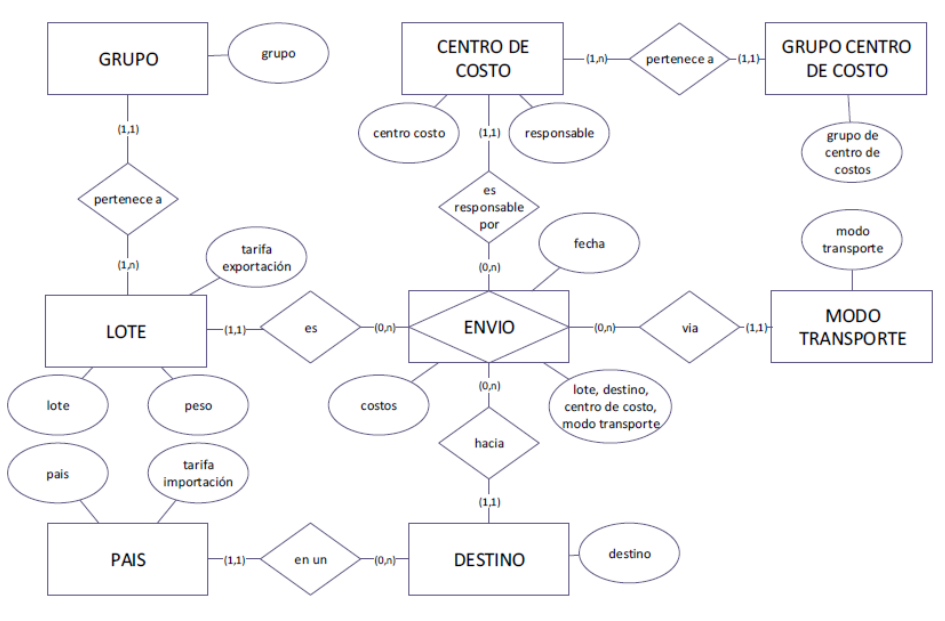
\includegraphics[width=12.5cm]{img/ejer1.png}  
\end{center}
Supongamos que los costos de los atributos ya incluyen todas las tarifas. No se transferirá más información sobre las tarifas
al almacén de datos. El análisis tendrá lugar a nivel del grupo de centros de costos, no se necesita información sobre los
centros de costos.
\\Por favor identifique el hecho de interés y construya el Modelo Dimensional y su respectivo diagrama físico
\begin{center}
    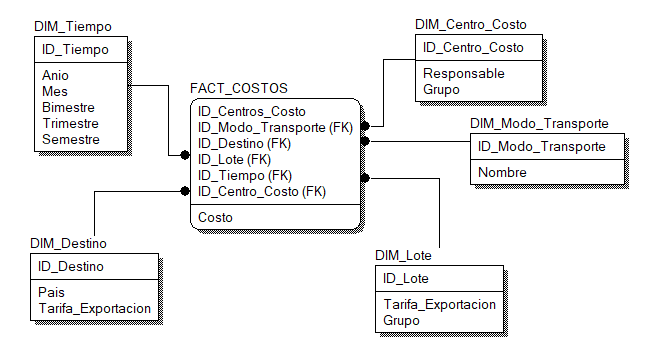
\includegraphics[width=15cm]{img/1.png}  
\end{center}

\subsection{Ejercicio 02: Reservas de viaje}
En este esquema de E / R, un cliente (que es de cierto tipo) reserva un viaje en una agencia de viajes. La agencia de viajes
trabaja para un determinado operador turístico. El viaje va a un destino determinado que pertenece a un país determinado.
\\La dimensión de tiempo consiste en mes, trimestre y año.
\begin{center}
    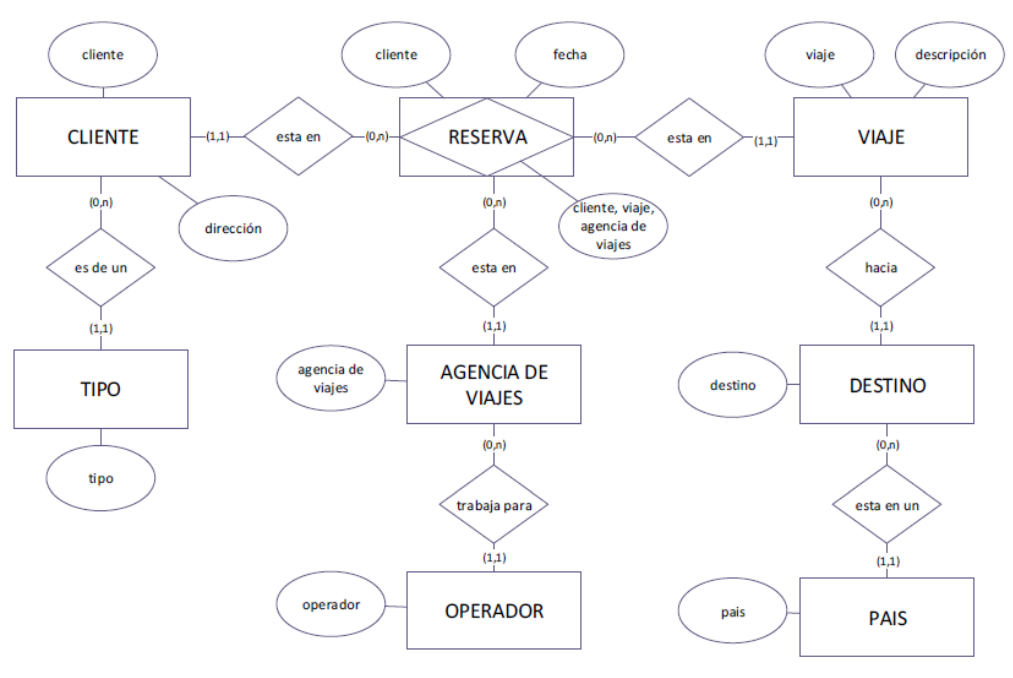
\includegraphics[width=12cm]{img/ejer2.png}  
\end{center}
Por favor identifique el hecho de interés y construya el Modelo Dimensional y su respectivo esquema físico.
\begin{center}
    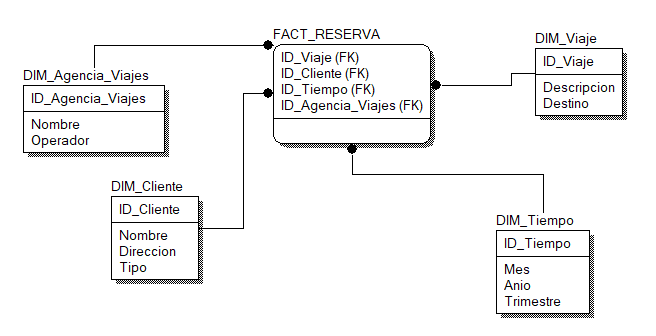
\includegraphics[width=15cm]{img/2.png}  
\end{center}


\subsection{Ejercicio 03: Gestión de proyectos}
Este esquema E / R simplificado muestra un caso gestión del proyecto.
\\El proyecto para un cliente se divide en varios paquetes de trabajo y siempre una persona es responsable de completar la
tarea. Se cuida en un lugar determinado.
\\La dimensión de tiempo consiste de día, mes y año
\begin{center}
    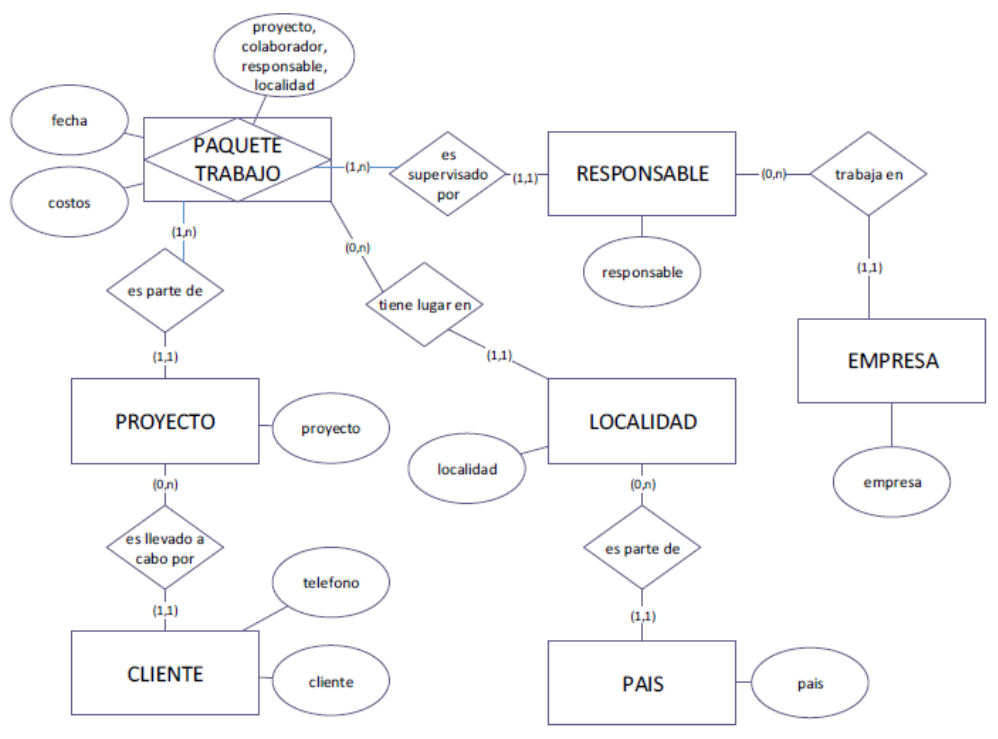
\includegraphics[width=14cm]{img/ejer3.png}  
\end{center}
Por favor identifique el hecho de interés y construya el Modelo Dimensional. Incluya un atributo de hecho adicional que
cuente la cantidad de paquetes de trabajo. Asimismo, realice el diagrama físico.
\begin{center}
    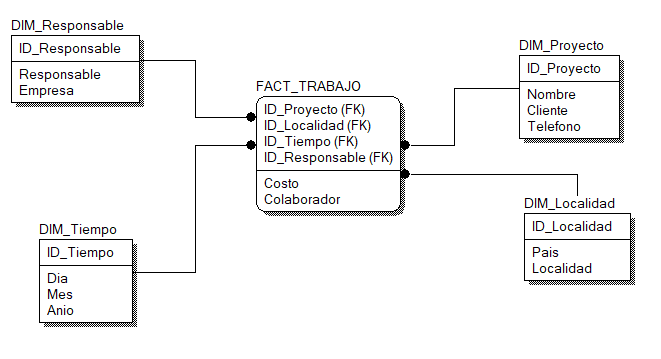
\includegraphics[width=15cm]{img/3.png}  
\end{center}



\end{document}

